\begin{spacing}{1.5}
	\begin{figure}[H]
		\centering
		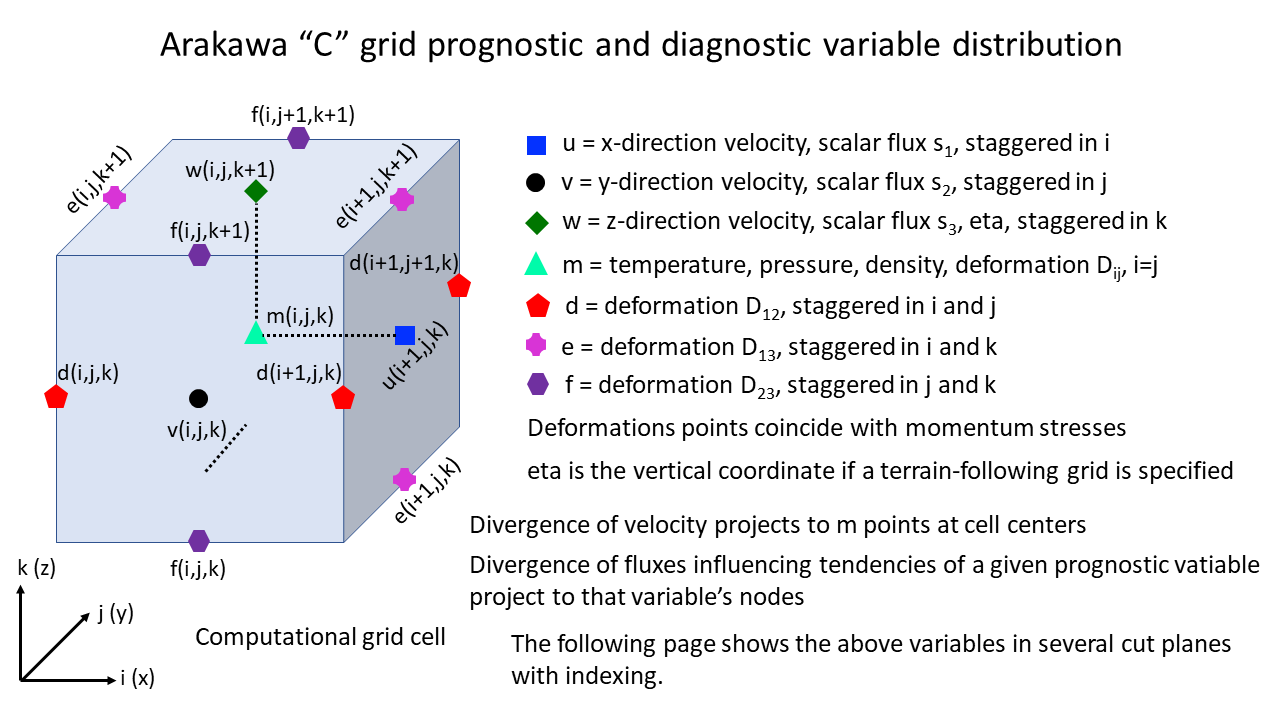
\includegraphics[width=1\textwidth]{contents/Arakawa_1.png}		
		\caption{Distribusi variabel pada C-grid Arakawa}
		\label{fig:arakawa_1}
	\end{figure}
	\begin{figure}[H]
		\centering
		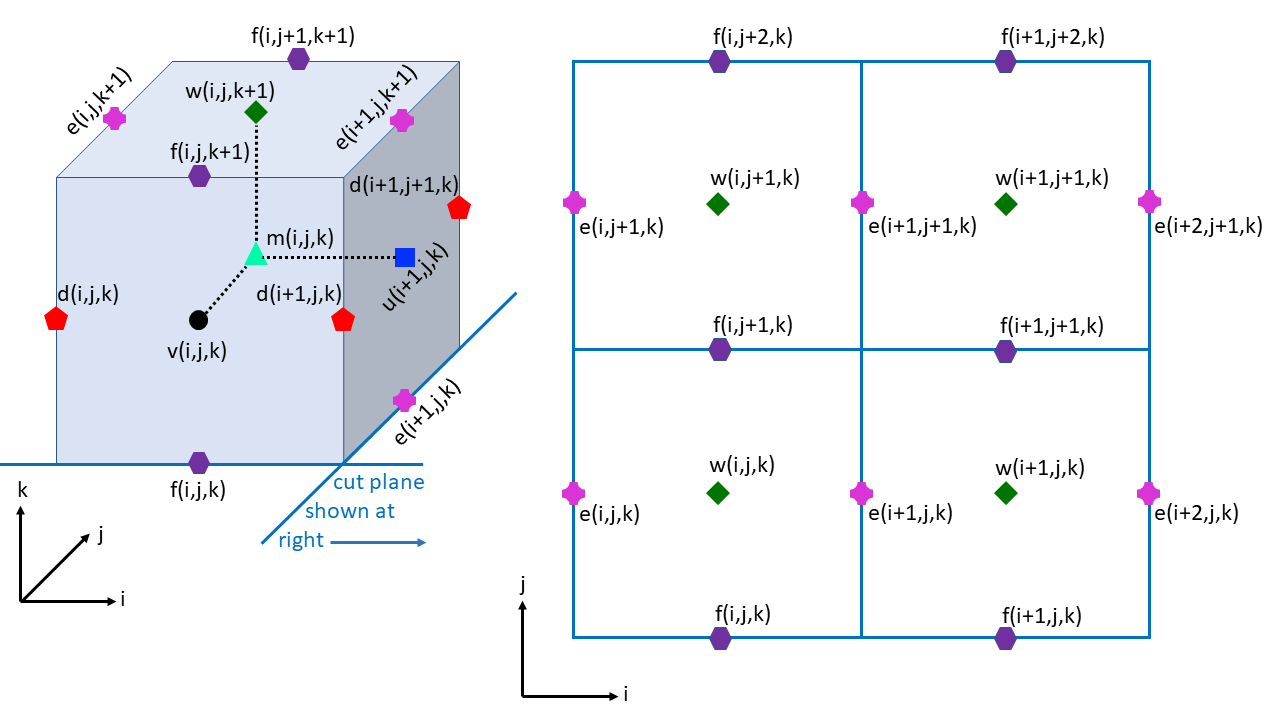
\includegraphics[width=1\textwidth]{contents/Arakawa_2.png}	
		\caption{Diskritisasi C-grid Arakawa (posisi bawah kubus, $k$ tetap)}
		\label{fig:arakawa_2}
	\end{figure}
	\begin{figure}[H]
		\centering
		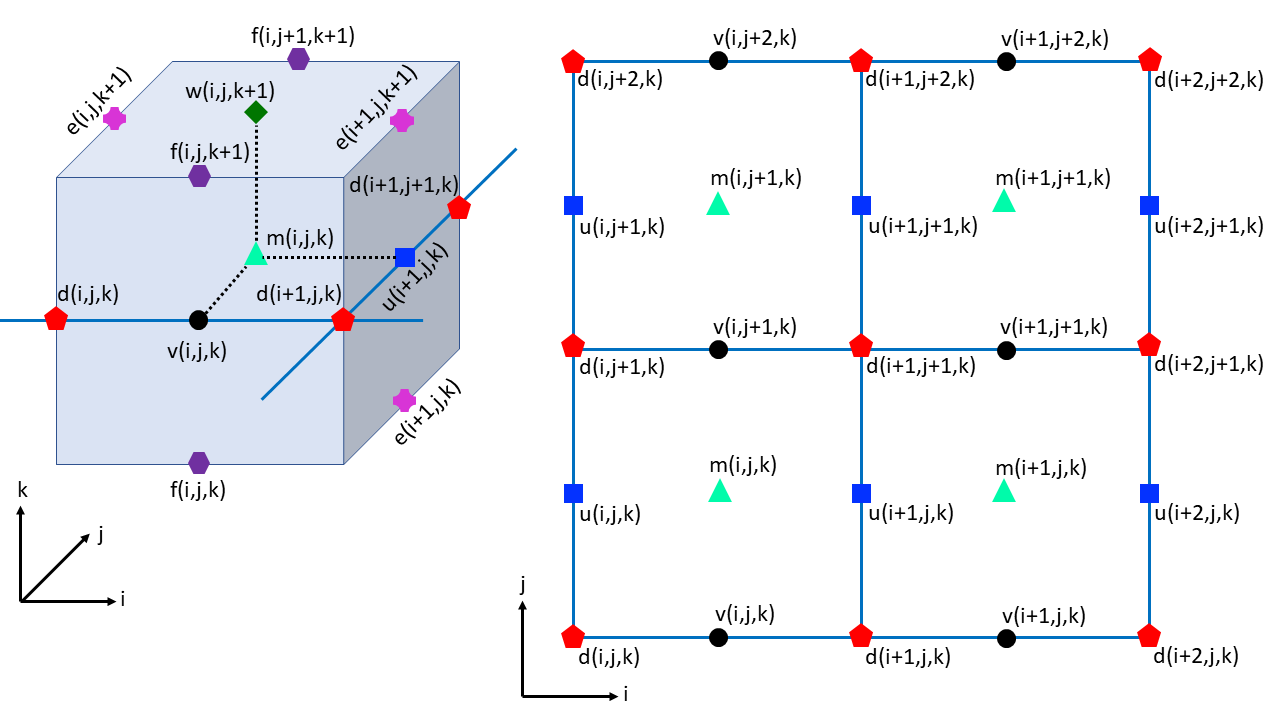
\includegraphics[width=1\textwidth]{contents/Arakawa_3.png}	
		\caption{Diskritisasi C-grid Arakawa (posisi tengah kubus, $k$ tetap)}
		\label{fig:arakawa_3}
	\end{figure}
		\begin{figure}[H]
		\centering
		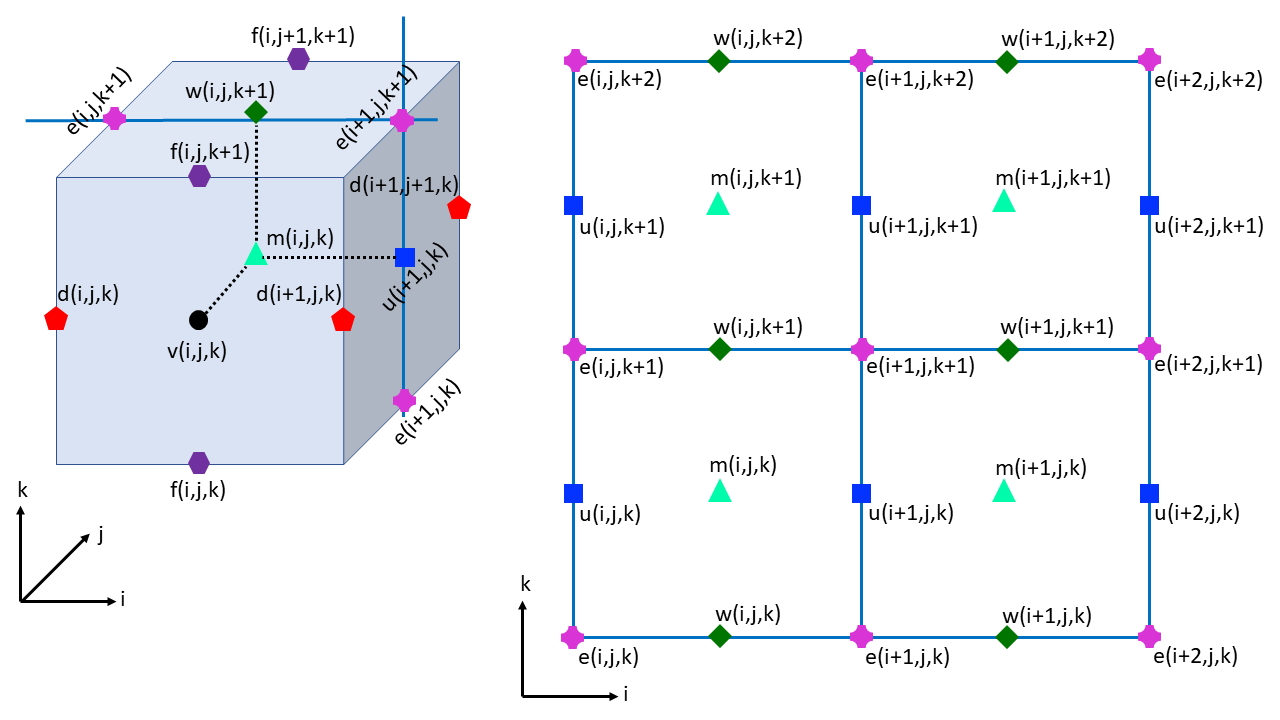
\includegraphics[width=1\textwidth]{contents/Arakawa_4.png}	
		\caption{Diskritisasi C-grid Arakawa ($j$ tetap)}
		\label{fig:arakawa_4}
	\end{figure}
		\begin{figure}[H]
		\centering
		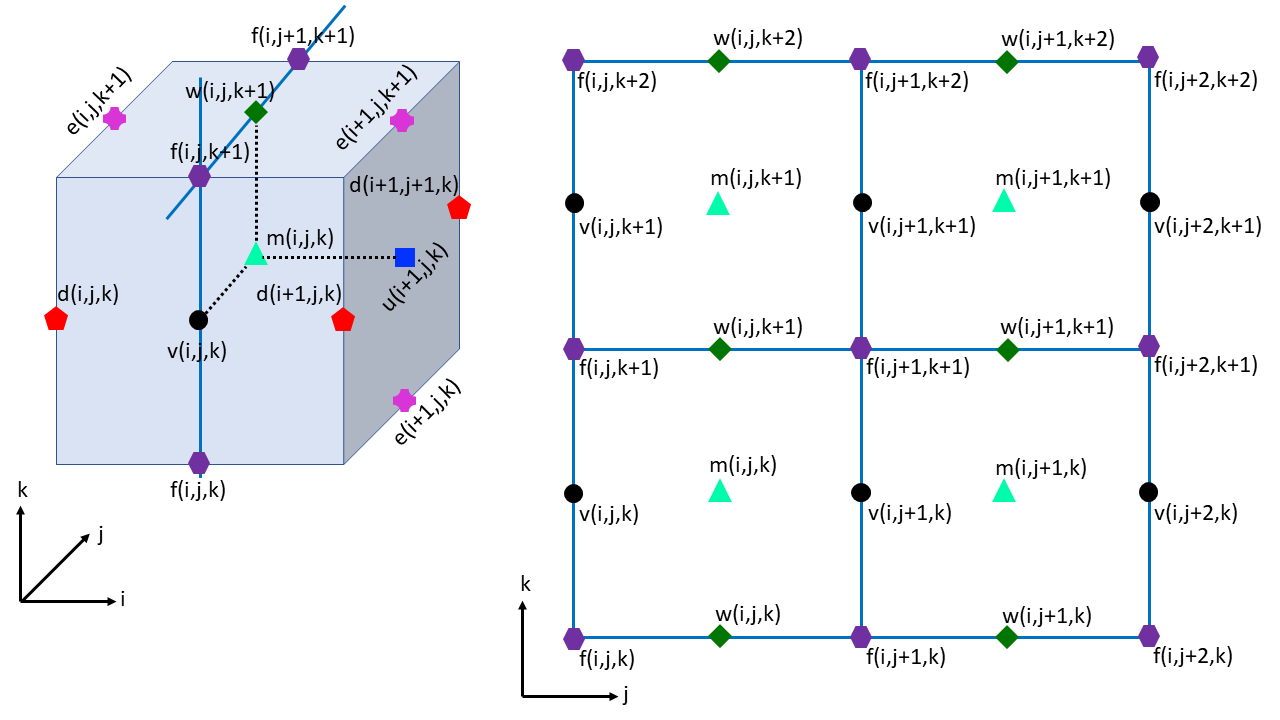
\includegraphics[width=1\textwidth]{contents/Arakawa_5.png}	
		\caption{Diskritisasi C-grid Arakawa ($i$ tetap)}
		\label{fig:arakawa_5}
	\end{figure}
\end{spacing}